% \documentclass[a4paper,11pt]{article}
% \usepackage[hyperref]{beamerarticle}

\documentclass[final]{beamer}

\usepackage[hangul]{kotex}
\usepackage{amsfonts,amsmath,xob-amssymb}

\usepackage{amsthm}
\newtheorem{defn}{Definition}
\newtheorem{thm}{Theorem}

\usepackage{cancel}
\graphicspath{{./_img/07/}}

\usepackage{graphicx}
\usepackage{media9}
\usepackage{tikz}
\usepackage{textpos}
\usepackage{multirow}

\mode<presentation>{
	\usetheme{Madrid}
	\usecolortheme{default}
	\usefonttheme{professionalfonts}
}

\def\b{\boldsymbol}

\mode<article>{
\usepackage{fullpage}
}
\usepackage{ulem}

\usepackage{mdframed}

\newcommand{\bb}{\mathbb}
\newcommand{\bd}{\mathbf}
\newcommand{\p}{\partial}

\newcounter{saveenumi}
\newcommand{\seti}{\setcounter{saveenumi}{\value{enumi}}}
\newcommand{\conti}{\setcounter{enumi}{\value{saveenumi}}}

\newcommand{\mail}{\url{mailto:experiment.namun+2016f@gmail.com} }


\title{진화게임이론}
\subtitle{게임이론과 진화의 만남}
\author[조남운]{허준석$\rightarrow$이동한$\rightarrow$\emph{조남운}\\\mail}

\begin{document}

\begin{frame}[t]{}
	\titlepage
\end{frame}
%--- Next Frame ---%

\begin{frame}[t]{목차}
	\tableofcontents
\end{frame}
%--- Next Frame ---%

\section{다윈주의와 진화} % (fold)
\label{sec:darwinism_and_evolution}

\begin{frame}[t]{Image of Evolution}
	\begin{columns}[c]
		\column{18em}
		\begin{itemize}
			\item The survival of fittest? 
			\item Darwin이 했던 말은 아니다! 다윈은 사실 진화라는 말도 쓰기를 꺼려 함. 
			\item 영국의 계관시인 테니슨(A. Tennyson): 자연은 ``피칠갑을 한 이빨과 발톱을 지니고 있다.''
			\item 허버트 스펜서가 적자생존이라는 말을 만들어 냄 
		\end{itemize}
		\column{13em}
		\hspace{-1em}
		\fbox{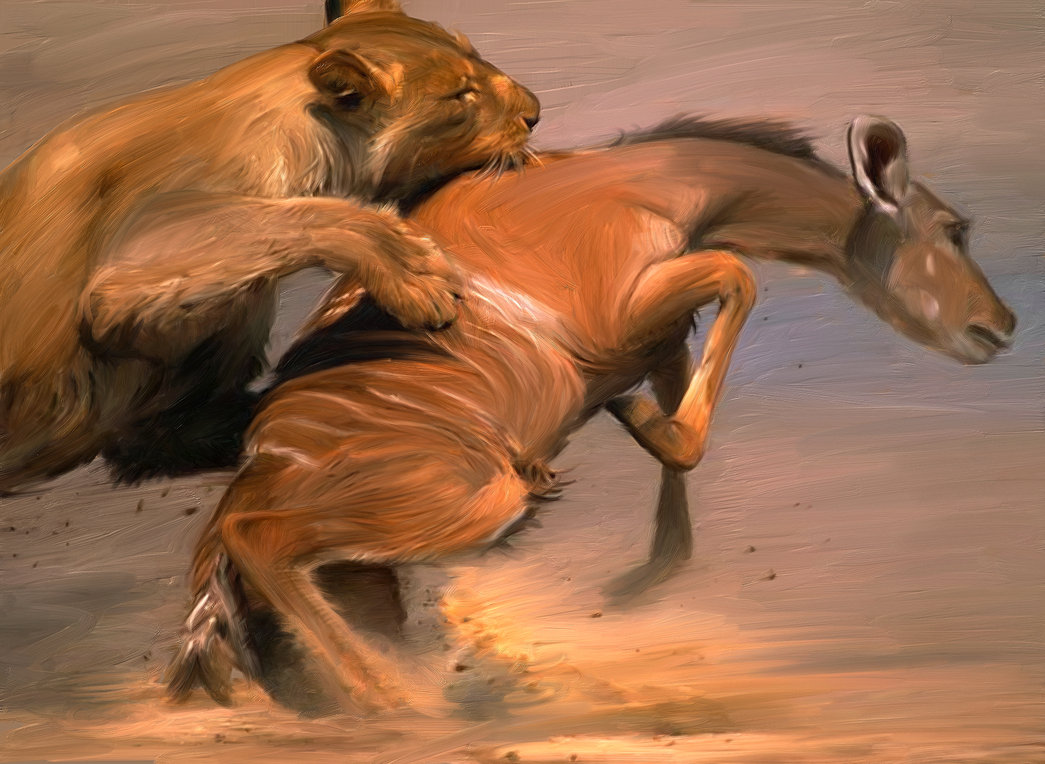
\includegraphics[width=13em]{Survival_of_the_Fittest_by_ApplePlus.jpg}}
	\end{columns}
\end{frame}
%--- Next Frame ---%

\begin{frame}[t]{Social Darwinism}
	\begin{columns}[c]
		\column{18em}
		\begin{itemize}
			\item 진화는 적자생존의 역사 
			\item 이에 따라서 사회는 진보한다. 
			\item 따라서 이에 대한 개입은 역사의 진보를 막는 것. 
			\item Hitler 등 나치와 파시즘에 기반을 제공 
			\item 현재까지 암묵적인 영향을 끼치고 있음 
		\end{itemize}
		\column{12em}
		%\hspace{-1em}
		\fbox{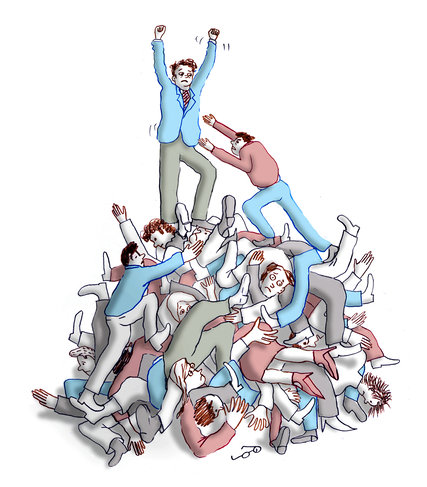
\includegraphics[width=11em]{social-darwinism.jpg}}
	\end{columns}
\end{frame}
%--- Next Frame ---%

\begin{frame}[t]{Social Darwinism}
	\begin{columns}[c]
		\column{18em}
		\begin{itemize}
			\item 무정부주의자 표트르 크로포트킨의 [상호부조론]
			\item ``Sociability is as much a law of nature as mutual struggle.''
			\item ``we at once see that those animals which acquire habits of mutual aid are undoubtedly the fittest. ''
		\end{itemize}
		\column{12em}
		%\hspace{-1em}
		\fbox{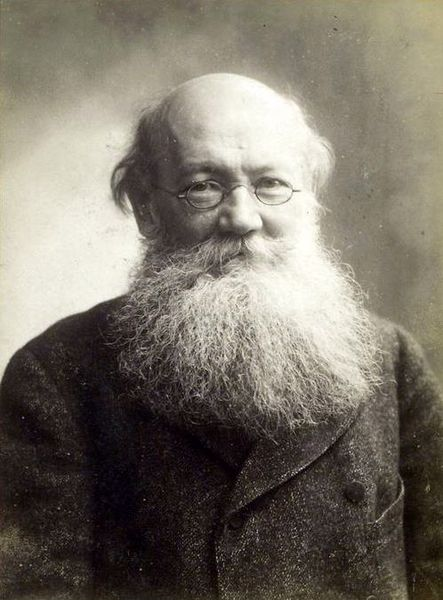
\includegraphics[width=11em]{Kropotkin.jpg}}
	\end{columns}
\end{frame}
%--- Next Frame ---%

\begin{frame}[t]{Nature's Best Achievement}
	\begin{columns}[c]
	\column{18em}
	\begin{itemize}
		\item 자연이 이룬 가장 놀라운 성과는 무엇일까? 
		\item 생명, 생명의 군집
		\item 이것은 모두 적자생존의 결과인가? \\
		아니면 또 다른 어떤 결과인가?
		\item 투쟁이 생명의 중요한 현상인 것은 분명하지만 뭔가 잊고 있는 것은 없을까?
	\end{itemize}
	\column{12em}
	\hspace{-1em}
	\fbox{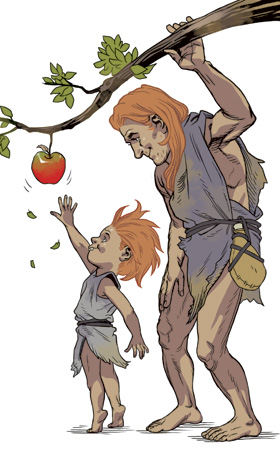
\includegraphics[width=11em]{Evolution-Cooperation_Dec.jpg}}
	\end{columns}
\end{frame}
%--- Next Frame ---%

\begin{frame}[t]{Human}
	\begin{columns}[c]
		\column{15em}
		\begin{itemize}
			\item 인간 개체를 생각해보자.
			\item 인간이라는 하나의 생명 개체는 여러 기관, 세포, 유전자 사이의 절묘한 협업에 의존 
			\item 만일 간 세포가 자신의 이익만을 이기적으로 추구한다면? 
			\item 결국 인간 자신이 적자생존에 반하는 존재
		\end{itemize}
		\column{16em}
		%\hspace{1em}
		\fbox{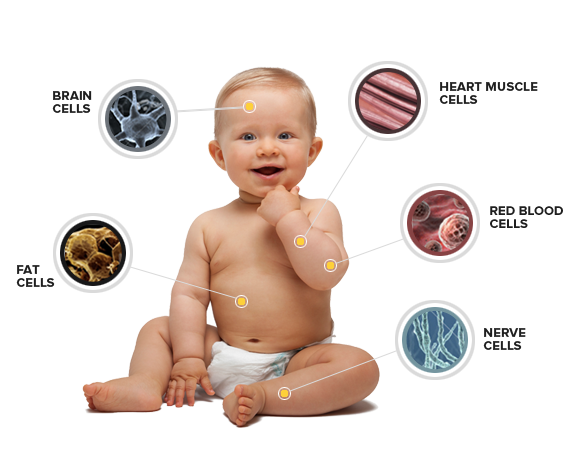
\includegraphics[width=15.5em]{human.png}}
	\end{columns}
\end{frame}
%--- Next Frame ---%

\begin{frame}[t]{Three Principles of Evolution I: Selection}
	\begin{columns}[c]
		\column{18em}
		\begin{itemize}
			\item Selection \\[1.5em]
			\begin{mdframed}[backgroundcolor=yellow]\small
			점진적이며 비무작위적인 과정으로, 그 성향(유전자)을 지니고 있는 존재들의 차별적인 재생산능력의 결과로서 이러한 생물학적 성향을 가진 개체가 집단에서 더 많아지거나 흔해지게 된다. 
			\end{mdframed}	
		\end{itemize}
		\column{13em}
		\fbox{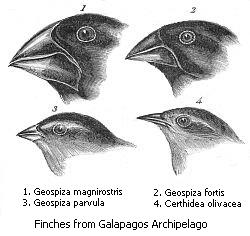
\includegraphics[width=13em]{Darwin_finches.jpeg}}
	\end{columns}
\end{frame}
%--- Next Frame ---%

\begin{frame}[t]{Three Principles of Evolution II: Mutation}
	\begin{columns}[c]
	\column{18em}
	\begin{itemize}
		\item Mutation \\[1.5em]
	\begin{mdframed}[backgroundcolor=yellow]\small
	유전학적으로, 유기체, 바이러스 혹은 염색체외 유전 요소가 지닌 게놈의 뉴클레오타이드 계열의 (임의적) 변화
	\end{mdframed}	
	\end{itemize}
	\column{13em}
	\fbox{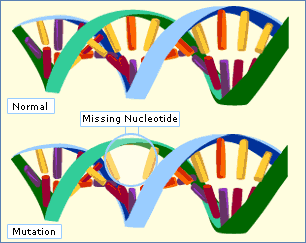
\includegraphics[width=13em]{DeletionMutationGEN.png}}
	\end{columns}
\end{frame}
%--- Next Frame ---%

\begin{frame}[t]{Three Principles of Evolution III: 종합}
	\begin{columns}[c]
		\column{18em}
		\begin{itemize}
			\item (자연)선택은 더 적합한 쪽으로의 움직임을 만들고  
			\item 변이는 일정한 상태의 안정성에 변화를 만든다. 
		\end{itemize}
		\column{13em}
		\hspace{-1em}
		\fbox{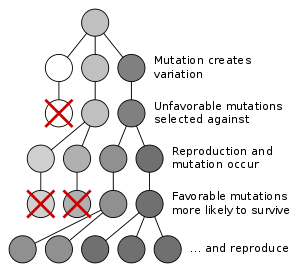
\includegraphics[width=13em]{mutationandselection.png}}
	\end{columns}
\end{frame}
%--- Next Frame ---%

\begin{frame}[t]{The Third Principle of Evolution}
	\begin{columns}[c]
		\column{18em}
		\begin{itemize}
			\item 협력은 선별의 결과이고, 협력에 반하는 변이에 안정성을 지녀야 한다. 
			\item 선별이 더 많은 자손을 남기는 것이라고 할 때
			\item 어떤 상황에서 왜 (자신의 이익에 반할 때에도) 협력하는가? 
			\item 게임이론이 도움을 준다! 
		\end{itemize}
		\column{13em}
		\fbox{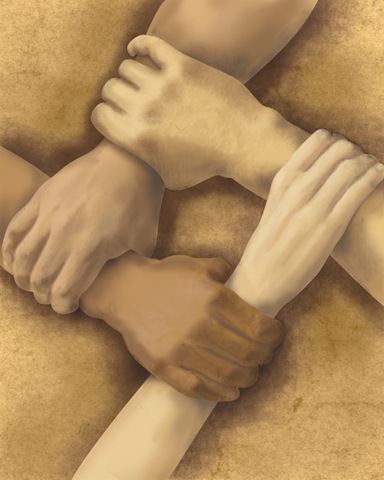
\includegraphics[width=12em]{cooperation_1.jpg}}
	\end{columns}
\end{frame}
%--- Next Frame ---%

\begin{frame}[t]{최재천 선생 강의 동영상}
	%\begin{columns}[c]
	%\column{18em}
	\begin{itemize}
		\item 다윈에 대한 개괄적인 이해를 위해서 \\
		\href{http://www.youtube.com/watch?v=hUSElnxxzF0}{LINK}
	\end{itemize}

	%\column{13em}
	%\fbox{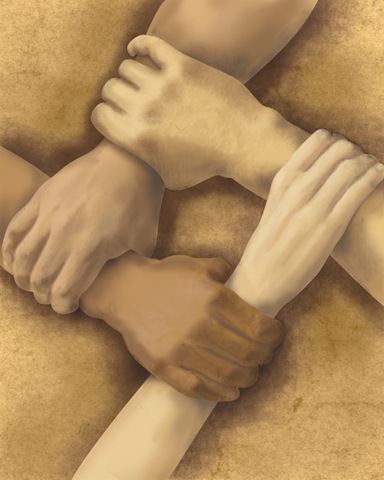
\includegraphics[width=12em]{cooperation_1.jpg}}
	%\end{columns}
\end{frame}
%--- Next Frame ---%

% section darwinism_and_evolution (end)

\section{진화게임이론} % (fold)
\label{sec:Evolutionary_Game_Theory}

\begin{frame}[t]{Evolution Meets Game Theory I}
	\begin{itemize}
		\item 지금까지 표준적인 게임이론에서 경지자들이 균형전략에 따라 행동하기 위한 전제는?
		\item 진화적 게임이론에서는 어떠한 합리성도 부여하지 않은 채 논의가 전개됨
		\item “프로그램화 되어 있는” 전략에 따라 경기자들이 행동  
		\item 동일한 전략을 갖고 태어난 경기자들 사이에서도 어떤 전략으로 프로그램되어 있는 경기자를 만나는가에 따라 다른 보수를 얻게 됨
		\item 전략이 확산되는 과정은 경기자들이 얻게 될 보수의 크기에 의존
		\item 구체적인 과정은 i 유전적 전수과정 ii 문화적 전수과정
	\end{itemize}
\end{frame}
%--- Next Frame ---%

\begin{frame}[t]{Evolution Meets Game THeory II}
	\begin{columns}[c]
		\column{15em}
		\begin{itemize}
			\item 게임이론은 원래 합리적 행위자의 이익추구에 동원되는 사고법
			\item 이것이 어떻게 맹목의 과정인 진화와 어울리게 되었을까?
			\item 결국 선별이란 주어진 집단(population)에서 어떤 개체가 더 나은 결과를 얻는지의 문제 
			%\item 만일 게임이론을 인구집단에 기반해 정의할 수 있다면?
		\end{itemize}
		\column{15em}
		\fbox{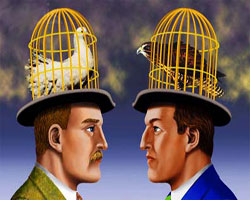
\includegraphics[width=14em]{hawk-and-dove.jpg}}
	\end{columns}
\end{frame}
%--- Next Frame ---%

\begin{frame}[t]{Elements of Evolutionary Game Thoery}
	\begin{columns}[c]
		\column{15em}
		\begin{itemize}
			\item 플레이어의 합리적 판단은 제거 혹은 제한 
			\item 게임은 집단에 기반하여 진행. 게임의 결과는 이 집단의 구성으로 반영된다.  
			\item 이러한 과정의 무한 반복은 어떤 결과를 낳을까? 
		\end{itemize}
		\column{15em}
		\hspace{-1em}
		\fbox{
\includegraphics[width=15em]{population-rainbow.jpg}}
	\end{columns}
\end{frame}
%--- Next Frame ---%

\begin{frame}[t]{Theory}
	\begin{itemize}
		\item $n$명으로 구성된 인구집단이 있다고 하자. 
		\\ (일단 $n$은 필요한 만큼 크다고 가정)
		\item 유형, 전략은 두 개만 있다고 가정
		\item 플레이어들은 일정한 시간별로 함께 게임을 벌인다. 
		\\ 예를 들어 5분 간격으로 한번씩 짝을 지워 게임을 한다. 
		\item 일정한 횟수의 상호작용이 있고 난 후 인구 집단에 속한 다른 플레이어들 혹은 다른 유형의 플레이어들의 보수를 관찰 
		\begin{enumerate}
		\item 만일 상대의 보수가 나보다 크다면, 그의 전략을 복제!
		\item 만일 상대의 보수가 나보다 작다면, 현재 전략을 고수!
		\end{enumerate}
	\end{itemize}
\end{frame}
%--- Next Frame ---%

\begin{frame}[t]{Payoff}
	\begin{columns}[c]
	\column{10em}
	%
	\begin{align*}
	\bordermatrix{%
	%& 0 & 1 & 2 \cr
	   & A & B \cr
	A & a & b  \cr
	B & c & d  \cr
	}
	\end{align*}
	%
	\column{21em}
	\hspace{-1em}
	\begin{itemize}
		\item 선수1과 선수2가 만난다. 
		\item 만일 선수1의 유형이 A이고 선수2가 B라면?
		\item 둘의 게임은 대칭적이기 때문에 
		\item 보수행렬은 옆과 같이 쓸 수 있다! 
	\end{itemize}
	\end{columns}
\end{frame}
%--- Next Frame ---%

\begin{frame}[t]{Replicator Dynamics}
	%
	\begin{align*}
	\underbrace{\dot{x_i}}_{1)} = x_i \underbrace{(\pi_i - \overline{\pi})}_{2)}
	\end{align*}
	%
	\begin{enumerate}
	\item $i$라는 특정한 전략이 얼마나 변화하는지를 나타낸다. 
	\item $i$라는 전략이 누리는 보수가 평균에 비해서 얼마나 큰지를 나타낸다. 
	\end{enumerate}
	%
	\vspace{2em}
	\begin{mdframed}[backgroundcolor=yellow]\small
	진화의 과정을 나타내는 방정식. $i$라는 전략/유형이 평균보다 큰 보수를 누릴수록, 그들의 숫자가 많을수록 그 증가폭도 커지게 된다. 
	\end{mdframed}	
	%
	
\end{frame}
%--- Next Frame ---%

\begin{frame}[t]{How to Get Payoff I}
	\begin{itemize}
		\item 두 유형 밖에 없으므로 $A$ 유형의 비율을 $x$라고 하면 $B$ 유형의 비율은 $1-x$
		\item 그리고 두 유형이 한 번의 게임을 통해서 얻을 수 있는 평균 보수는 
		\begin{align*}
		\pi_A & = a x + b (1-x) \\
		\pi_B & = c x + d (1-x) 
		\end{align*}
		\item 전체의 평균보수 $\overline{\pi}$는 어떻게 구할까? 
		\begin{align*}
		x {\,} \pi_A + (1-x) \pi_B
		\end{align*}
	\end{itemize}
\end{frame}
%--- Next Frame ---%

\begin{frame}[t]{How to Get Payoff II}
	\begin{itemize}
	\item 따라서, 
	%
	\begin{align*}
	\dot{x}=x(1-x)\underbrace{\left[ (a-b-c+d)x + b-d \right]}_{(\ast)}
	\end{align*}
	%
	\item 만일 $0<x<1$이라면, $x(1-x)$는 양수이므로, 이 게임에서 특정한 유형이 증감 여부는 $(\ast)$가 결정!
	\item $(\ast)$의 움직임에 따라서 게임을 몇 가지로 구분할 수 있다. 일단
	%
	\begin{align*}
	x^* = \frac{d-b}{a-b-c+d}
	\end{align*}
	%
	\end{itemize}
\end{frame}
%--- Next Frame ---%

\begin{frame}[t]{Dominance}
	\begin{columns}[c]
	\column{17em}
	\begin{itemize}
	\item 앞서 배웠던 우월전략을 떠올려보자. 
	\item 즉, $a<c$ 그리고 $b<d$ (B가 우월전략) $\rightarrow$ $\{(a-b-c+d)x + b-d \} < 0$
	$\rightarrow$ $\dot{x} < 0$ $\rightarrow$ A$\downarrow$
	%\item 전자의 경우 $A$가 $B$에 비해서 항상 우월 
	\item 그렇다면, $x=1$과 $x=0$ 중에 `안정적'인 것은?
	\end{itemize}
	\column{14em}
	\hspace{-1em}
	\fbox{
\includegraphics[width=14em]{arrowsD01.png}}
	\begin{table}
	\setlength{\tabcolsep}{1.2em}
	\begin{tabular}{|c|c|c|c|} \hline
	&  {A(C)} & {B(D)} \\ \hline
	{A(C)} & {$3$}, {$3$} & {$1$}, {$4$} \\ \hline%
	{B(D)} & {$4$}, {$1$} & {$2$}, {$2$} \\ 
	\hline
	\end{tabular}
	\end{table}
	%
	\begin{align*}
	\bordermatrix{%
	%& 0 & 1 & 2 \cr
	   & A & B \cr
	A & a & b  \cr
	B & c & d  \cr
	}
	\end{align*}
	%
	\end{columns}
\end{frame}
%--- Next Frame ---%

\begin{frame}[t]{Bistability}
	\begin{columns}[c]
		\column{17em}
		\small
		\begin{itemize}
		\item 만일 $a>c$ 그리고 $d>b$ 라면... 앞서 배운 어떤 게임과 비슷한가??
		\item MSNE? $1 \cdot x + 0 \cdot (1-x) = 0 \cdot x + 2 \cdot (1 - x)$ $\rightarrow$ $x = \frac{2}{3}$
		\item $\{(a-b-c+d)x + b-d \} > 0$ (즉, $\dot{x} > 0$) 가 되려면, $x > \frac{2}{3}$
		\item $x=1$과 $x=0$ 중에 `안정적'인 것은?
		\item $x^*$의 역할은? 
		\item 앞서 배웠던 내시 균형과는 어떻게 다른가? 
		\end{itemize}
		\column{14em}
		\hspace{-1em}
		\fbox{
\includegraphics[width=14em]{arrowsB01.png}}
		\begin{table}
		\setlength{\tabcolsep}{1.2em}
		\begin{tabular}{|c|c|c|c|} \hline
		& {A(L)} &  {B(R)}\\ \hline
		{A(L)} & {$1$}, {$1$} & {$0$}, {$0$} \\ \hline%
		{B(R)} & {$0$}, {$0$}  & {$2$}, {$2$}\\ 
		\hline
		\end{tabular}
		\end{table}
	\end{columns}
\end{frame}
%--- Next Frame ---%

\begin{frame}[t]{Co-existence}
	\begin{columns}[c]
		\column{17em}
		\small
		\begin{itemize}
		\item 만일 $a<c$ 그리고 $d<b$ 라면?
		\item 앞서 배운 어떤 게임과 비슷한가? 
		\item MSNE? $\frac{1}{2} \cdot x + 0 \cdot (1-x) = 1 \cdot x - \frac{1}{2} \cdot (1 - x)$ $\rightarrow$ 
		$x = \frac{1}{2}$
		\item $\{(a-b-c+d)x + b-d \} > 0$ (즉, $\dot{x} > 0$) 가 되려면, $x < \frac{1}{2}$
		\item $\dot{x} > 0$ if $x < \frac{1}{2}$, $\dot{x} < 0$ if $x > \frac{1}{2}$
		\item $x=1$과 $x=0$ 중에 `안정적'인 것은?
		\item $x^*$의 역할은?
		\item 앞서 배웠던 내시 균형과는 어떻게 다른가? 
		\end{itemize}
		\column{14em}
		\hspace{-1em}
		\fbox{\includegraphics[width=14em]{arrowsc01.png}}
		\begin{table}
		\setlength{\tabcolsep}{1.2em}
		\begin{tabular}{|c|c|c|c|} \hline
		&  {A(H)} & {B(D)} \\ \hline
		{A(H)} & {$-\frac{1}{2}$}, {$-\frac{1}{2}$} & {$1$}, {$0$} \\ \hline%
		{B(D)} & {$0$}, {$1$} & {$\frac{1}{2}$}, {$
		\frac{1}{2}$}\\ 
		\hline
		\end{tabular}
		\end{table}
	\end{columns}
\end{frame}
%--- Next Frame ---%

\begin{frame}[t]{Neutrality}
	\begin{columns}[c]
		\column{17em}
		\begin{itemize}
		\item 만일 $a=c$ 그리고 $d=b$ 라면?
		\item 앞서 배운 어떤 게임과 비슷한가? 
		\item $x=1$과 $x=0$ 중에 `안정적'인 것은?
		\item $x^*$의 역할은?
		\item 앞서 배웠던 내시 균형과는 어떻게 다른가? 
		\end{itemize}
		\column{14em}
		\hspace{-1em}
		\fbox{
\includegraphics[width=14em]{arrowsN01.png}}
		\begin{table}
		\setlength{\tabcolsep}{1.2em}
		\begin{tabular}{|c|c|c|c|} \hline
		& {A} &  {B}\\ \hline
		{A} & {$1$}, {$1$} & {$3$}, {$1$} \\ \hline%
		{B} & {$1$}, {$3$}  & {$3$}, {$3$}\\ 
		\hline
		\end{tabular}
		\end{table}
	\end{columns}
\end{frame}
%--- Next Frame ---%

\begin{frame}[t]{What Stability?}
	\begin{columns}[c]
	\column{20em}
	\begin{itemize}
	\item 우리는 암묵적으로 ``안정성''이라는 개념을 썼다. 
	\item 이 개념은 앞서 배운 진화의 두 개념과 연결해서 생각해보자. 
	\item 선택은 어느 쪽으로 나아갈지를 결정한다. 
	\item 변이는 그 나아감이 멈추었을 때 그 멈춤이 지속될 것인지를 결정
	\item Evolutionarily stable strategy\\진화적으로 안정적인 전략 
	\end{itemize}
	\column{11em}
	\hspace{-1em}
	\fbox{
\includegraphics[width=11em]{neutral.png}}
	\end{columns}
\end{frame}
%--- Next Frame ---%

% section Evolutionary_Game_Theory (end)

\section{협력으로 가는 길} % (fold)
\label{sec:Road_to_Cooperation}

\begin{frame}[t]{그러나 진화적인 관점만으로는!}
	\begin{itemize}
	\item 죄수의 딜레마는 해결할 수 없다! \\(대단히 표준적인 가정 아래 있다면...)
	\end{itemize}
	\begin{center}
	\fbox{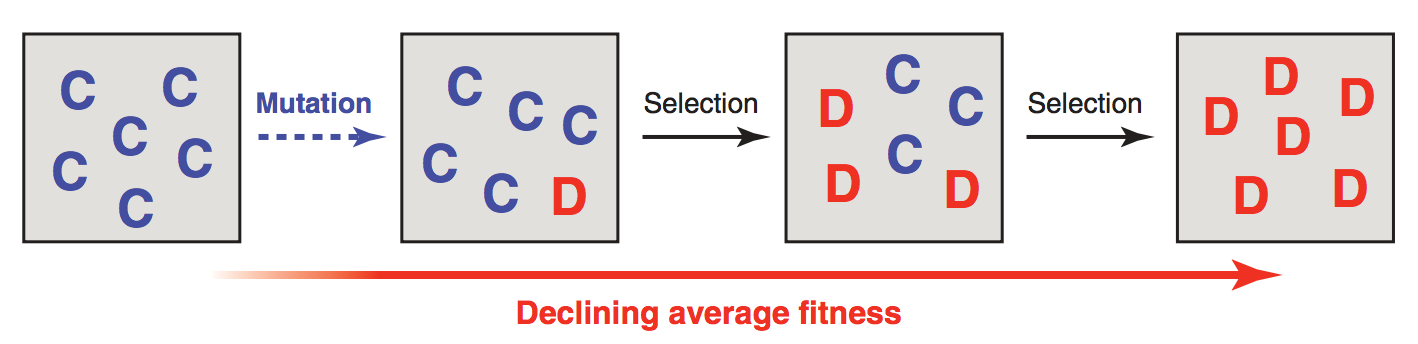
\includegraphics[width=30em]{decline.png}}
	\end{center}
\end{frame}
%--- Next Frame ---%

\begin{frame}[t]{Solving PD Game}
	\begin{columns}[c]
		\column{20em}
		\begin{itemize}
		\item 대표적으로 쓰이는 보수행렬
		\item 두 명이 대칭적이므로 한 명의 보수만 쓰자.
		\item $b$: 이득(benefit), $c$: 비용(cost) 
		\item 딜레마가 되려면? $b>c$
		\end{itemize}
		\column{15em}
		\begin{align*}
		\bordermatrix{%
		%& 0 & 1 & 2 \cr
		   & C & D \cr
		C & b-c & -c  \cr
		D & b & 0  \cr
		}
		\end{align*}
	\end{columns}
\end{frame}
%--- Next Frame ---%

\begin{frame}[t]{Martin Nowak}
	\begin{columns}[c]
	\column{20em}
	\begin{itemize}
	\item 협력의 진화를 터준 5가지 경로 혹은 변형\\(물론, 유일하거나 절대적인 것은 아니야!)
	\item 게임이론을 통한 통일적 접근 
	\item 협력에 관한 최신의 (쉽고?) 수학적인 지도의 완성
	\end{itemize}
	\column{12em}
	\fbox{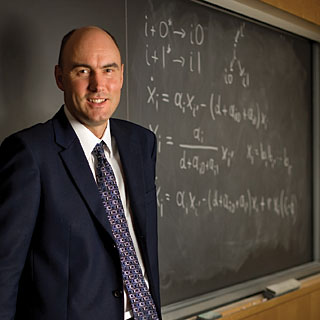
\includegraphics[width=10em]{nowak_2.jpg}}
	\end{columns}
\end{frame}
%--- Next Frame ---%

\begin{frame}[t]{한 눈에 보는 5가지 길}
	\begin{columns}[c]
	\column{10em}
	\fbox{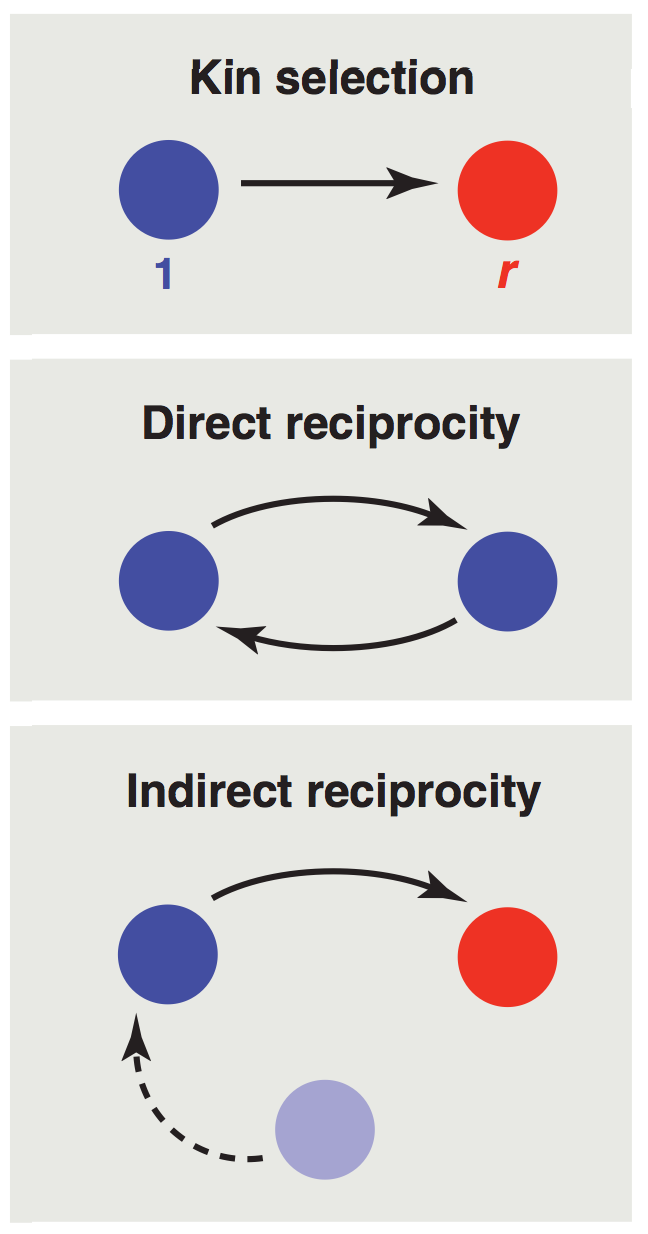
\includegraphics[width=10em]{five_1.png}}
	\column{20em}
	\vspace{-1em}
	\begin{itemize}
	\item ``네 이익이 나의 이익과 같다면'' (Kin Selection)\\[4em]
	\item ``네가 나를 돕는다면'' (Direct Reciprocity)\\[5em]
	\item ``그이가 저이를 도왔기에'' (Indirect Reciprocity) 
	\end{itemize}
	\end{columns}
\end{frame}
%--- Next Frame ---%

\begin{frame}[t]{한 눈에 보는 5가지 길 (2)}
	\begin{columns}[c]
	\column{10em}
	\fbox{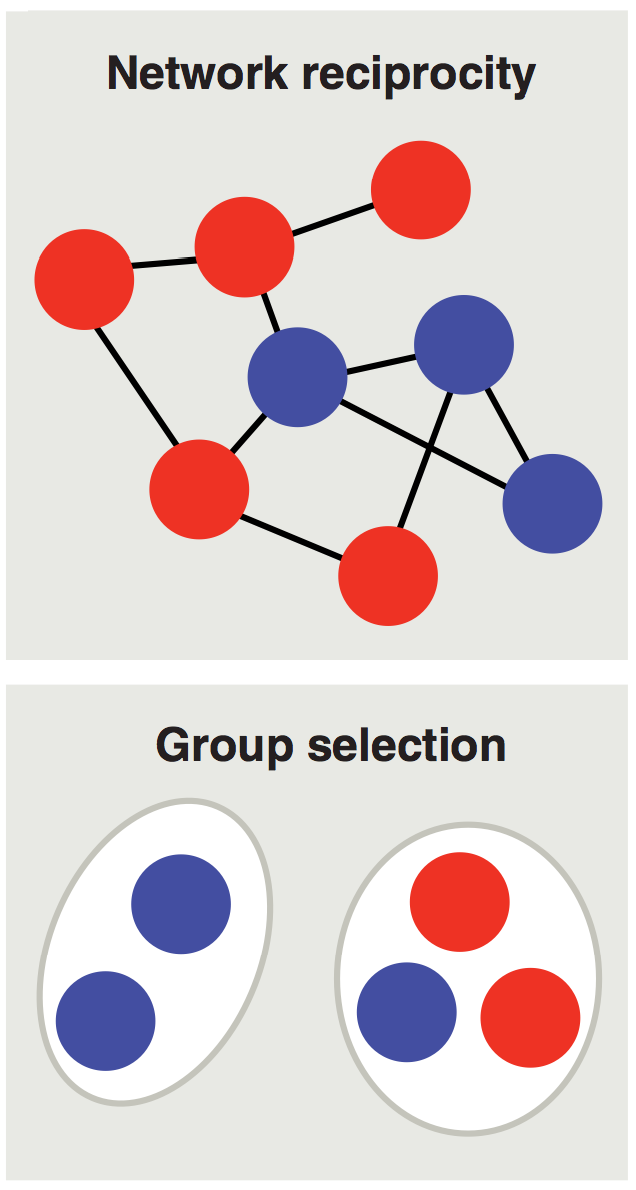
\includegraphics[width=10em]{five_2.png}}
	\column{20em}
	\vspace{0em}
	\begin{itemize}
	\item ``그들이 나와 같다면'' (Network Reciprocity)\\[8em]
	\item ``우리가 그들을 물리칠 수 있다면'' (Group Selection)
	\end{itemize}
	\end{columns}
\end{frame}
%--- Next Frame ---%

\begin{frame}
  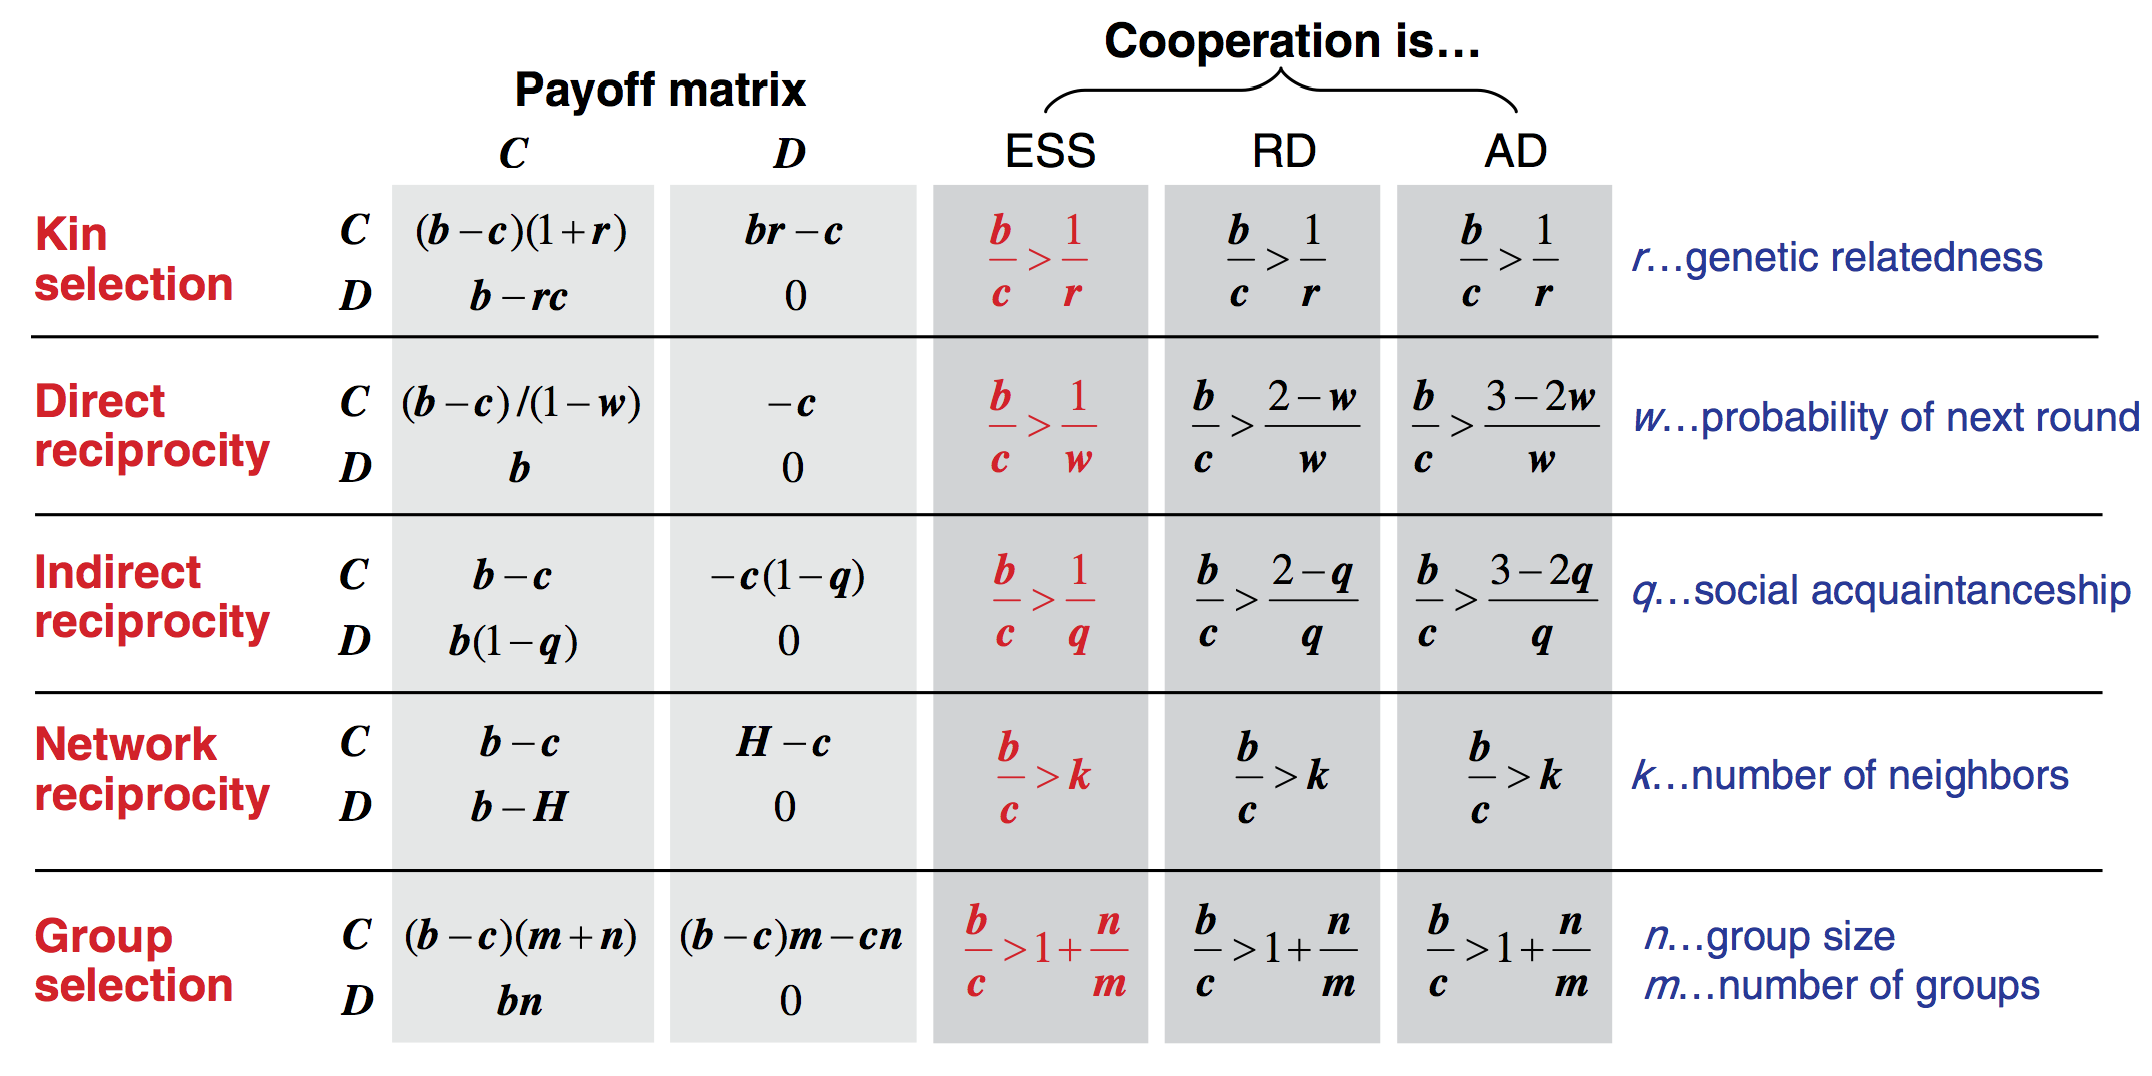
\includegraphics[width=\textwidth]{fiverule.png}
\end{frame}

\begin{frame}[t]{Evolution of Cooperation I: Kin Selection}
	\begin{columns}[c]
	\column{20em}
	\begin{itemize}
	\item 형제 혹은 자매와 협력하는 이유: 친족이 같은 유전자를 지니고 있을 가능성이 높기 때문  
	\item 리처도 도킨스의  "이기적 유전자"
	\item 매트 리들리의 "이타적 유전자"
	\item 두 가지 방식으로 진행
	\begin{enumerate}
	\item 자손의 번식을 통해서 
	\item 동일한 유전자를 지니고 있는 친척의 번식을 높임으로써 
	\end{enumerate}
	\end{itemize}
	\column{12em}
	\fbox{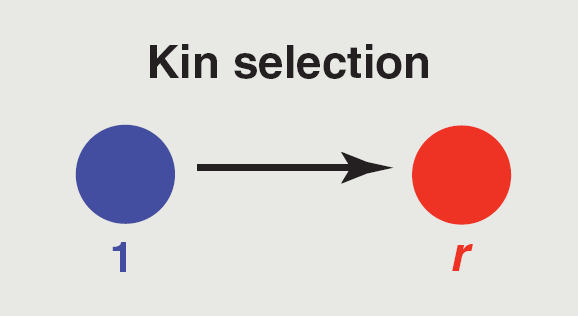
\includegraphics[width=10em]{kinselection.png}}
	\end{columns}
\end{frame}
%--- Next Frame ---%

\begin{frame}[t]{Evolution of Cooperation II: Direct Reciprocity}
	\begin{columns}[c]
	\column{20em}
	\begin{itemize}
	\item 오밀조밀한 공동체 
	\item 다른이에 대한 나의 경험에 기반 
	\item 반복게임을 통해서 
	\end{itemize}
	\column{12em}
	\fbox{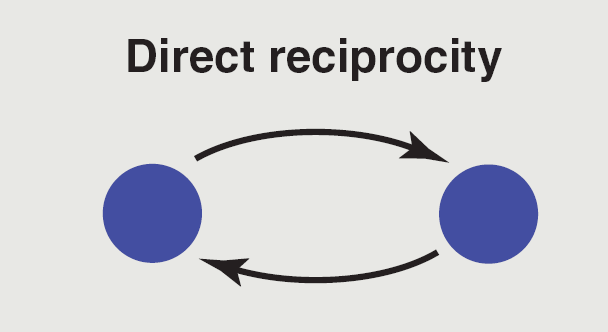
\includegraphics[width=10em]{directreciprocity.png}}
	\end{columns}
\end{frame}
%--- Next Frame ---%

\begin{frame}[t]{Evolution of Cooperation III: Indirect Reciprocity}
	\begin{columns}[c]
	\column{20em}
	\begin{itemize}
	\item 대규모 사회(이 거대한 사회가 굴러가는 방식) $\rightarrow$ 사회적 분업 
	\item 다른이에 대한 다른 사람의 경험 또한 고려 
	\item 언젠가 만날 수 있겠지? 
	\item "뇌"의 진화와 평판을 매개로
	\item 도덕체계의 진화 (그리스 철학, 불교, 기독교, 힌두교, 도교 등)
	\end{itemize}
	\column{12em}
	\fbox{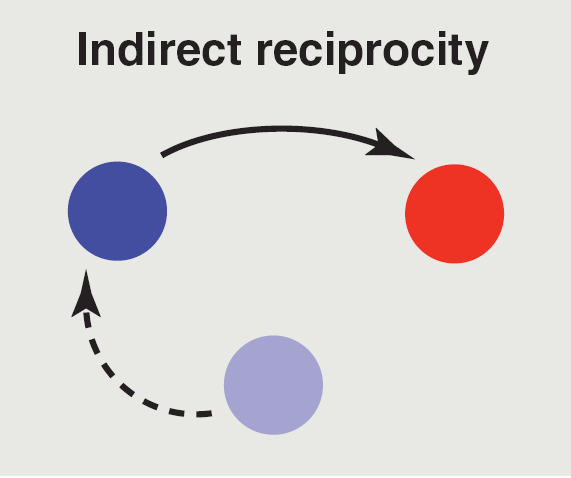
\includegraphics[width=10em]{indirectreciprocity.png}}
	\end{columns}
\end{frame}
%--- Next Frame ---%

\begin{frame}[t]{Evolution of Cooperation IV: Network Reciprocity}
	\begin{columns}[c]
	\column{20em}
	\begin{itemize}
	\item 집단의 구조가 죄수의 딜레마를 푸는 또 다른 방법을 제시할 수 있지 않을까? 
	\item 현실의 모든 상태에는 일정한 구조가 있다. 이것이 차이를 낳을까?
	\item 어떻게 얼룩말의 세포들이 얼룩말의 무늬를 만들어 내는 가? 
	\item 협력자가 배신자 보다 더 나은 성과를 거두게 하는 그런 집단 구조가 있을까?
	\end{itemize}
	\column{12em}
	\fbox{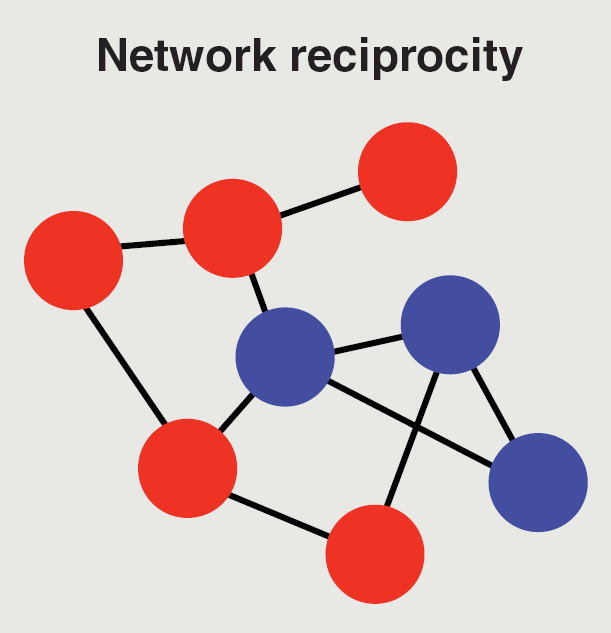
\includegraphics[width=10em]{network.png}}
	\end{columns}
\end{frame}
%--- Next Frame ---%

\begin{frame}[t]{Network Reciprocity}
	\begin{columns}[c]
	\column{20em}
	\begin{itemize}
	\item Conway's The Game of Life: 두 가지 규칙 
	 \begin{enumerate}
	\item 중앙 셀의 주변에 2개 미만 혹은 3개 초과의 셀들이 살아 있으면 중앙 셀이 죽도록 한다.
	\item 중앙 셀의 주변에 정확히 3개의 셀들이 살아 있으면 중앙 셀이 다시 살아나도록 한다. 
	\end{enumerate}
	\end{itemize}
	\column{12em}
	\fbox{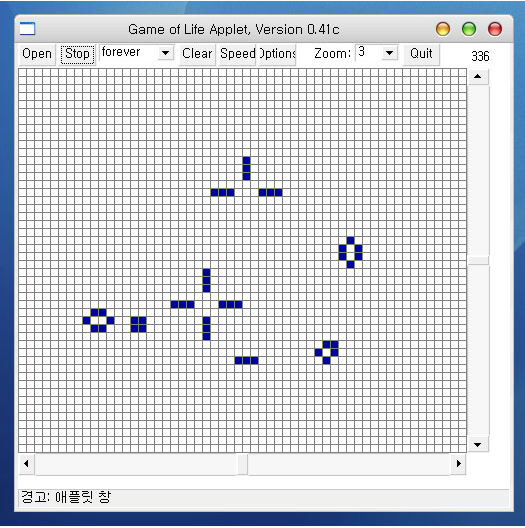
\includegraphics[width=10em]{gameoflife.png}}
	\end{columns}
\end{frame}
%--- Next Frame ---%

\begin{frame}[t]{Network Reciprocity (2)}
	\begin{columns}[c]
	\column{15em}
	\begin{itemize}
	\item Spatial Games
	 \begin{enumerate}
	\item 그림의 각 셀들이 주변에 있는 8개의 이웃 셀들과 게임을 벌인다. 
	\item 각 선수(셀)들의 보수가 계산되고 각 선수들은 이웃 셀 중에서 가장 보수가 높은 셀을 모방한다.
	\item 초기의 상태에 따라서 결과는 달라진다. 
	\end{enumerate}
	\end{itemize}
	\column{17em}
	\fbox{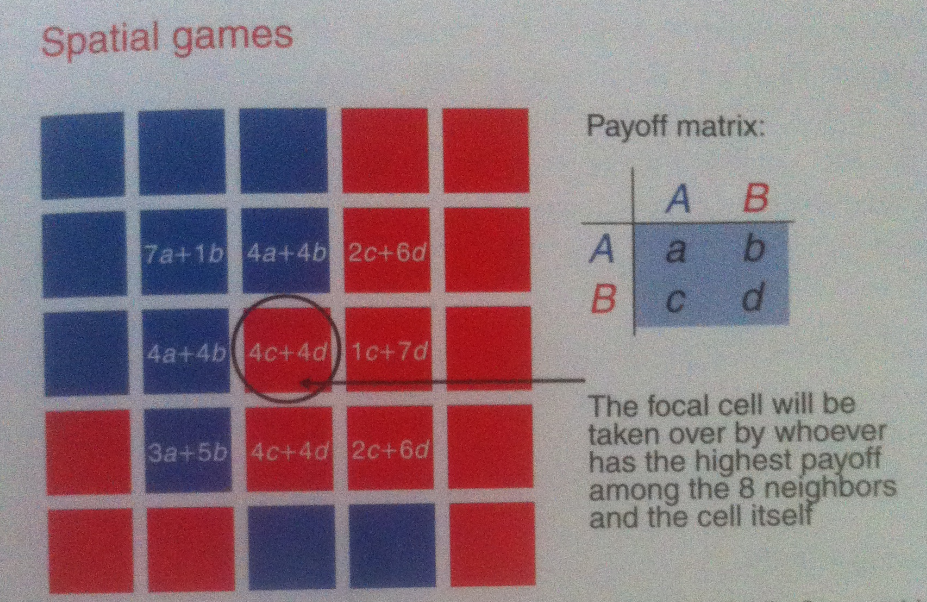
\includegraphics[width=15em]{spatialgames.png}}
	\end{columns}
\end{frame}
%--- Next Frame ---%

\begin{frame}[t]{Evolution of Cooperation V: Group Selection}
	\begin{columns}[c]
		\column{20em}
		\begin{itemize}
		\item 집단은... 지하철 선로에 떨어진 어린 아이를 구한 학생에게 상장과 존경을 제공한다.
		\item 바람직한 사회규범을 가진 집단은 그렇지 않은 집단들과의 경쟁에서 승리할 것이다.
		\item 간접 상호성은 집단 선택과 협력하여 인간다움을 형성할 수 있다.
		\end{itemize}
		\column{12em}
		\fbox{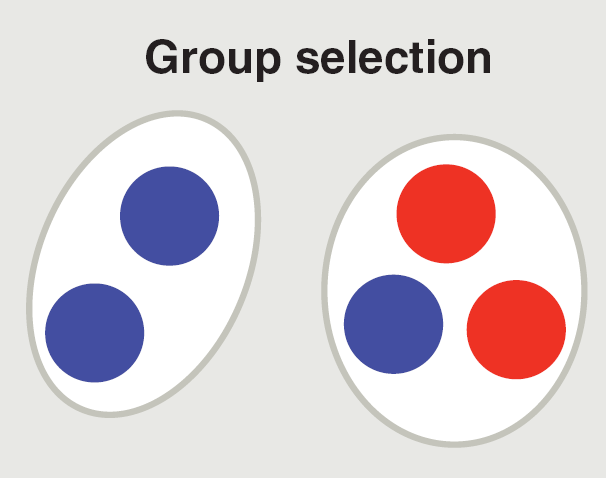
\includegraphics[width=10em]{groupselection.png}}
	\end{columns}
\end{frame}
%--- Next Frame ---%

\begin{frame}[t]{Direct Reciprocity: Oscillations of Cooperation and Defection}
	\begin{columns}[c]
	\column{15em}
	\begin{itemize}
		\item 진화에서 협력의 역할을 이해하는 중요한 게임은 PDG
		\item PDG에서 협력은 없어지고 배신은 증가 
		\item Repeated PDG는 직접적 상호성(Direct Reciprocity)을 이해하는 주요한 분석틀 $\rightarrow$ 협력이 진화하는 메커니즘을 보여준다. 
	\end{itemize}
	\column{15em}
	\fbox{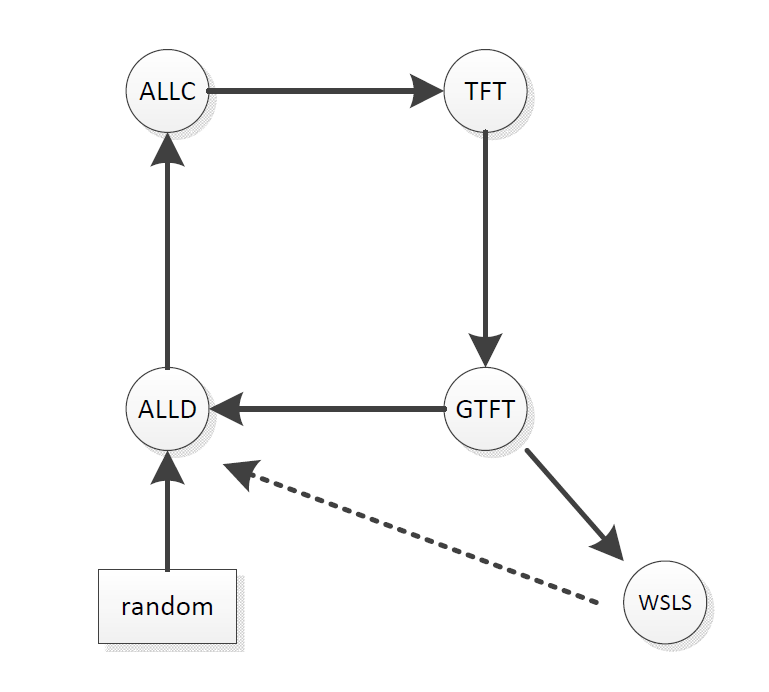
\includegraphics[width=14em]{dynamics01.png}}
	\end{columns}
\end{frame}
%--- Next Frame ---%

\begin{frame}[t]{Cyclic Pattern}
	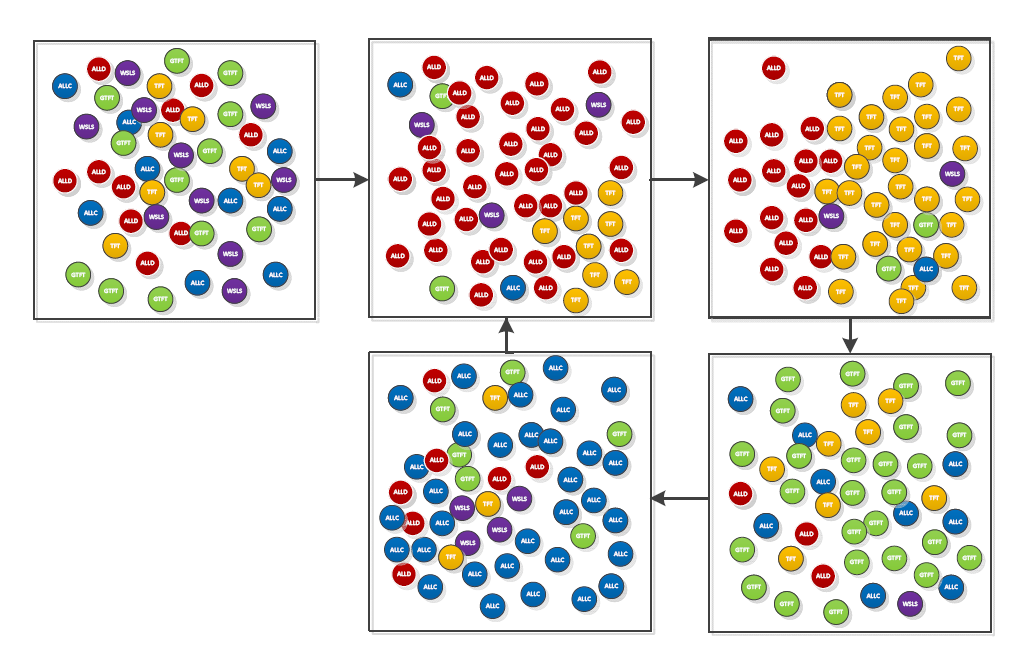
\includegraphics[width=\textwidth]{cyclicpattern01.png}
\end{frame}
%--- Next Frame ---%

% section Road_to_Cooperation (end)

\end{document}